%clase del documento
\documentclass[a4paper,12pt]{article}

%paquete de idioma y codificación de caracteres
\usepackage[spanish]{babel}
\usepackage[utf8]{inputenc}

% soporte gráfico
\usepackage{graphicx}
\graphicspath{ {images/} }

%datos del documento
\title{Anteproyecto de Trabajo de Fin de Grado}
\author{Ignacio Agüero Salcines}


\begin{document}
	
	\maketitle
	
	\newpage
	
	{\Large Contexto del proyecto}\\
	
Esta es una empresa que se dedica al consulting informático,y que dentro de ella, se desarrolla LUCA.\\


 LUCA es un producto que abstrae al usuario de las consultas a las diversas fuentes de datos (ya sean servicios, bases de datos, o similar) bajo un único lenguaje común. Este producto permite crear y gestionar consultas.\\


 Actualmente surge la necesidad de poder anidar los diversos procesos\footnote{Un proceso se explica como una entidad que por sí misma tiene la capacidad de realizar llamadas a servicio para recoger datos en función de unas variables de entrada y de salida.} independientes entre sí, así como la dificultad para organizarlos, interactuar y ejecutarlos.\\
	
	Este proyecto pretende crear un componente de procesos genérico, el cual será capaz de crear diagramas donde el usuario enlace sea capaz de enlazar los diferentes procesos entre sí, utilizando para ello variables de entrada y de salida, así como ejecutarlos y obtener respuestas de ellos.\\
	
	Entre las características que se le exigen es que sea lo mas configurable posible y estar preparado para posibles incrementos futuros.
	Además se pretende que dicho proyecto sea fácil de usar e intuitivo, es decir, altamente usable.\\
	
	Este componente será capaz de proveer una soporte gráfico (mediante una herramienta o motor gráfico llamado GO.JS) y lógico para llevar a cabo la funcionalidad final.\\
	
	A parte del componente genérico, se pretende realizar una integración en una aplicación ya existente, donde se incorporara la funcionalidad descrita. Demostrará así su fácil integración y usabilidad.\\
	
	\newpage
	{\Large Arquitectura y/o tecnologías del proyecto}\\
	
	El componente genérico se compone de dos soportes principales, uno mediante la herramienta javascript GO.JS, el cuál se encargara de visualizar gráficamente los datos (aunque también contiene una lógica interna propia a desarrollar), y otro soporte lógico encargado presentar el patrón MVP (modelo vista presentador), que interactuará con la herramienta gráfica.\\
	
	\begin{center}
		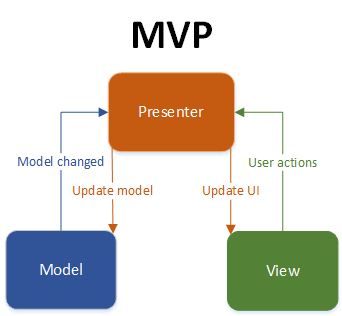
\includegraphics{images/mvp}\\
	\end{center}
	
	
	Este ensamblado de herramientas se realizará usando Vaadin, el cuál, mediante un fichero conector escrito en javascript, se encargará de realizar las comunicaciones entre la parte lógica y la parte gráfica.\\
	
	
	\begin{center}
		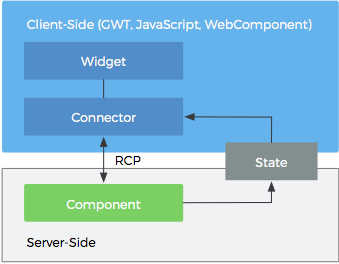
\includegraphics{images/schema}\\
	\end{center}
	

	
\end{document}